\documentclass[conference]{IEEEtran}
\IEEEoverridecommandlockouts
% The preceding line is only needed to identify funding in the first footnote. If that is unneeded, please comment it out.
\usepackage{cite}
\usepackage{amsmath,amssymb,amsfonts}
\usepackage{algorithmic}
\usepackage{graphicx}
\usepackage{textcomp}
\usepackage{xcolor}
\usepackage[brazilian]{babel}
\usepackage[utf8]{inputenc}
\usepackage[T1]{fontenc}
\usepackage{listings}
\usepackage{color}
\usepackage{float}
\usepackage{multirow}

\definecolor{dkgreen}{rgb}{0,0.6,0}
\definecolor{gray}{rgb}{0.5,0.5,0.5}
\definecolor{mauve}{rgb}{0.58,0,0.82}

\lstset{frame=tb,
  language=Java,
  aboveskip=3mm,
  belowskip=3mm,
  showstringspaces=false,
  columns=flexible,
  basicstyle={\small\ttfamily},
  numbers=none,
  numberstyle=\tiny\color{gray},
  keywordstyle=\color{blue},
  commentstyle=\color{dkgreen},
  stringstyle=\color{mauve},
  breaklines=true,
  breakatwhitespace=true,
  tabsize=3
}
\lstset{language=Python}
\def\BibTeX{{\rm B\kern-.05em{\sc i\kern-.025em b}\kern-.08em
    T\kern-.1667em\lower.7ex\hbox{E}\kern-.125emX}}
\begin{document}

\title{Relatório do Laboratório 4: \\ Otimização com Métodos Baseados em População\\
}

\author{\IEEEauthorblockN{Isabelle Ferreira de Oliveira}
\IEEEauthorblockA{\textit{CT-213 - Engenharia da Computação 2020} \\
\textit{Instituto Tecnológico de Aeronáutica (ITA)}\\
São José dos Campos, Brasil \\
isabelle.ferreira3000@gmail.com}
}

\maketitle

\begin{abstract}
Esse relatório documenta a implementação do algoritmo de otimização baseado em população: \textit{Particle Swarm Optimization} (PSO). Esse método foi testado tanto na otimização de uma função simples, para verificar o correto funcionamento do PSO, quanto na otimização dos parâmetros do controlador de um robô seguidor de linha.
\end{abstract}

\begin{IEEEkeywords}
Algoritmos de Otimização, população, \textit{Particle Swarm Optimization} (PSO), robô seguidor de linha
\end{IEEEkeywords}

\section{Introdução}
Otimização consiste em encontrar o mínimo (ou máximo) de uma função, ou seja, encontrar o conjunto de parâmetros que levem essa função ao seu mínimo (ou máximo). Também pode ser visto como encontrar a melhor solução dentre todas as soluções viáveis. Nesses problemas de otimização também é possível haver restrições acerca dos parâmetros que serão analisados.

Dentre os mais diversos tipos de algoritmos de otimização, existem os métodos baseado em população. Esses métodos mantêm uma população de possíveis soluções, a fim de tentar encontrar diferentes mínimos locais da função a ser analisada, melhorando assim as chances de se obter uma solução promissora. Um exemplo famoso de algoritmo de otimização baseado em população é o \textit{Particle Swarm Optimization} (PSO).

O pseudo-código desse algoritmo pode ser visto na subseção a seguir. Em seguida, será apresentado como esse algoritmo foi implementado no contexto do laboratório.

\subsection{Particle Swarm Optimization (PSO)}
Será considerado uma classe \textit{ParticleSwarmOptimization}, representando o algoritmo PSO. Além disso, o pseudocódigo do uso do algoritmo a partir dessa classe é o mostrado a seguir. Nesse pseudocódigo, \textit{pso} é o objeto da classe \textit{ParticleSwarmOptimization}.

\begin{lstlisting}
for i in range(num_evaluations):
	position = pso.get_position_to_evaluate()
	value = quality_function(position)
	pso.notify_evaluation(value)
\end{lstlisting}

No pseudocódigo acima, \textit{quality\underline{\space}function()} é a função a ser maximizada. Assim, iterativamente por tantas vezes até se atingir uma convergência satisfatória ao(à) programador(a), o algoritmo calculará o valor da função para cada partícula na população de candidatas à solução. Para cada partícula, então, após esse cálculo, a função \textit{notify\underline{\space}evaluation()} compara o resultado obtido aos obtidos anteriormente a fim de encontrar o valor maximizado. Uma ideia de implementação em pseudocódigo da função \textit{notify\underline{\space}evaluation()} foi apresentada a seguir.

\begin{lstlisting}
def notify_evaluation(value):
	current_particle = get_current_particle_to_evaluate()

	if value > current_particle.my_best_value:
		current_particle.my_best_value = value
		current_particle.my_best_position = current_particle.position

	if value > global_best_value:
		global_best_value = value
		global_best_position = current_particle.position

	num_particle_evaluated = num_particle_evaluated + 1
	if num_particle_evaluated == num_particles:
		num_particle_evaluated = 0
		advance_generation()
\end{lstlisting}

\begin{lstlisting}
def advance_generation():
	for particle in particles:
		r_p = random.uniform(0, 1)
		r_g = random.uniform(0, 1)

		particle.velocity = inertia_weight * particle.velocity + cognitive_parameter * r_p * (particle.my_best_position - particle.position) + social_parameter * r_g * (global_best_position - particle.position)

		for i in range(quantity_of_dimensions):
			delta = upper_bound[i] - lower_bound[i]
    		particle.velocity[i] = min(max(particle.velocity[i], -delta), delta)
		
		particle.position = particle.position + particle.velocity

		for i in range(quantity_of_dimensions):
    		particle.position[i] = min(max(particle.position[i], lower_bound[i]), upper_bound[i])
\end{lstlisting}

\section{Implementação dos algoritmos}
Na parte relativa a implementação dos algoritmos de otimização, era necessário preencher os códigos das funções \textit{gradient\underline{\space}descent()}, \textit{hill\underline{\space}climbing()} e \textit{simulated\underline{\space}annealing()} do código base fornecido \cite{b1}.  Além disso, era necessário completar também os códigos das funções \textit{neighbors()} (para o método Hill Climbing), \textit{random\underline{\space}neighbor()} e \textit{schedule()} (para o método Simulated Annealing). 

A análise de vários pontos dos algoritmos descritos acima terão uma breve descrição em alto nível da sua implementação a seguir. 

Primeiramente, foi criada uma função \textit{check\underline{\space}stopping\underline{\space}condition()}, que, a partir do valor da função de custo naquele determinado teste, de um limite mínimo aceitável para essa função de custo, além dos números de iterações máximos aceitáveis e qual o atual número de iteração, decidia se era situação de parar o algoritmo ou não.

As funções \textit{J} apresentadas nos pseudo códigos acima se referiam a própria função de custo para cada um dos métodos e a função \textit{dJ} ao gradiente dessa função (esse já fornecido pelo código base).

Já a função \textit{neighbors()} retornava um \textit{array} de parâmetros vizinhos ao parâmetro analisado nessa determinada iteração, e esses vizinhos eram calculados conforme descrito no roteiro do laboratório \cite{b1}, utilizando as projeções no eixo X e Y (calculadas em Python a partir de \textit{numpy.cos()} e \textit{numpy.sin()}) para encontrar as coordenadas de cada vizinho.

A função \textit{random\underline{\space}neighbor()} foi implementada de forma análoga. A grande diferença foi, ao invés de retornar um \textit{array} de vizinhos, retornava apenas um, e o ângulo para as projeções foi obtido aleatoriamente de forma uniforme a partir da função de Python \textit{random.uniform(-numpy.pi, numpy.pi)}.

A função \textit{schedule()} seguiu a ideia fornecida pelo roteiro \cite{b1}. Assim, essa função retornava em Python \textit{temperature0/(1 + beta * (i ** 2))}.

Por fim, as funções \textit{gradient\underline{\space}descent()}, \textit{hill\underline{\space}climbing()} e \textit{simulated\underline{\space}annealing()} foram implementadas conforme apresentado nos pseudo códigos da seção Introdução, com alguns detalhes como armazenar toda a trajetória dos métodos adicionando os parâmetros \textit{theta} testados a cada iteração na lista \textit{history}. Além disso, para o caso do Hill Climbing, foram adicionadas condições específicas relativas ao caso no qual a variável \textit{best} ainda fosse \textit{None}. 

\section{Resultados e Conclusões}
Os resultados das trajetórias de otimização obtidos após a execução das implementações dos algoritmos descritos acima foram apresentados nas Figuras \ref{gradient_descent}, \ref{hill_climbing} e \ref{simulated_annealing} para Descida do Gradiente, Hill Climbing e Simulated Annealing, respectivamente, e a sobreposição dessas trajetórias foi apresentada na Figura \ref{optimization_comparison} para melhor comparação visual.

\begin{figure}[htbp]
\centering
\centerline{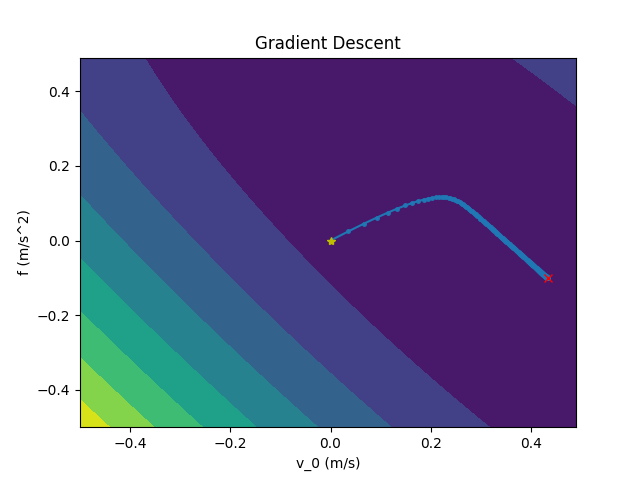
\includegraphics[scale=0.4]{gradient_descent.png}}
\caption{Trajetória de otimização usando Descida do Gradiente.}
\label{gradient_descent}
\end{figure}

\begin{figure}[htbp]
\centering
\centerline{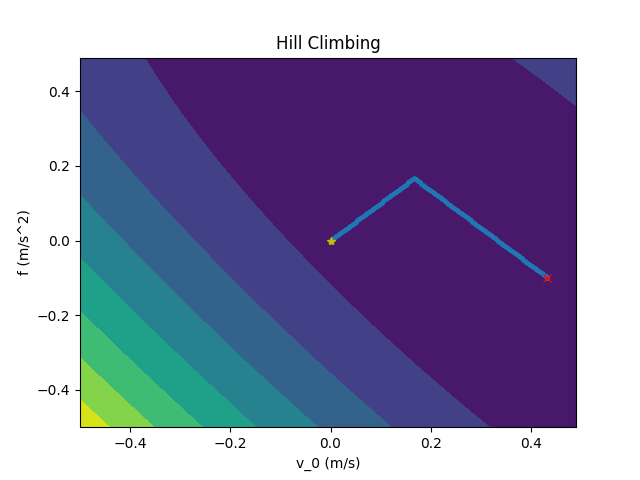
\includegraphics[scale=0.4]{hill_climbing.png}}
\caption{Trajetória de otimização usando Hill Climbing.}
\label{hill_climbing}
\end{figure} 

\begin{figure}[htbp]
\centering
\centerline{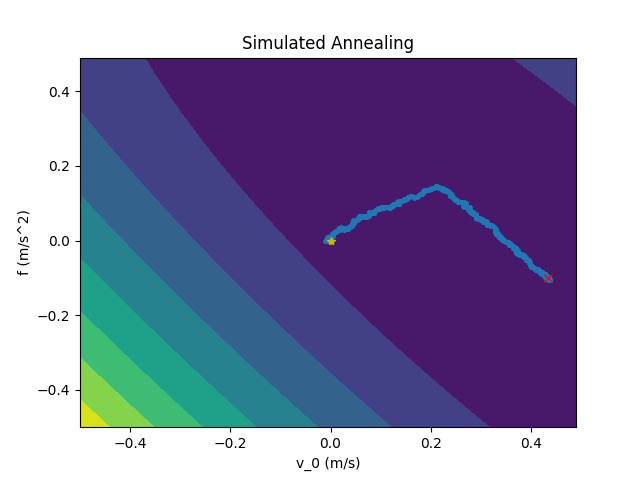
\includegraphics[scale=0.4]{simulated_annealing.png}}
\caption{Trajetória de otimização usando Simulated Annealing.}
\label{simulated_annealing}
\end{figure}

\begin{figure}[htbp]
\centering
\centerline{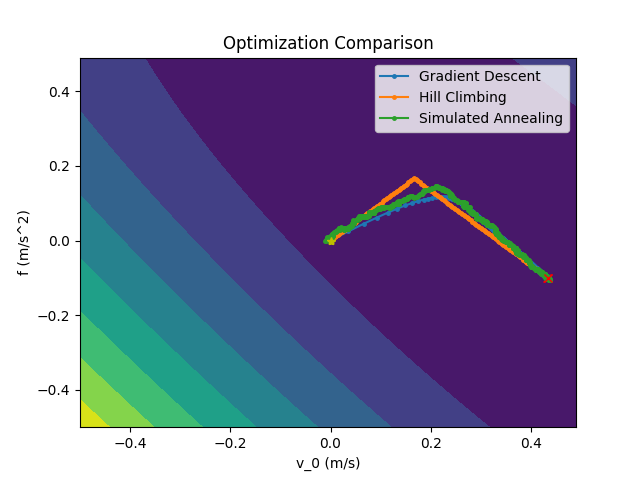
\includegraphics[scale=0.4]{optimization_comparison.png}}
\caption{Comparação de trajetórias de otimização usando Descida do Gradiente, Hill Climbing e Simulated Annealing.}
\label{optimization_comparison}
\end{figure}

Aplicando os valores encontrados para os parâmetros $v_0$ e $f$, o gráfico de velocidade da bola por tempo foi apresentado na Figura \ref{fit_comparison}. Esses valores numéricos de $v_0$ e $f$ podem ser vistos na Tabela \ref{tabelaX} para cada método estudado nesse laboratório, além do resultado fornecido inicialmente para o método de Mínimos Quadrados.

\begin{figure}[H]
\centering
\centerline{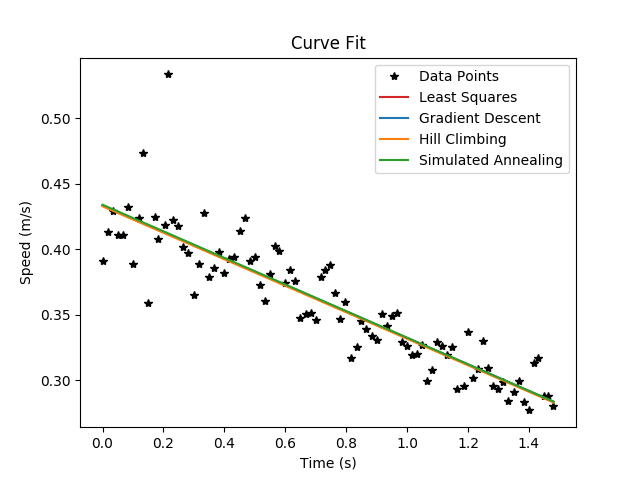
\includegraphics[scale=0.4]{fit_comparison.png}}
\caption{Comparação das regressões lineares das otimizações usando Descida do Gradiente, Hill Climbing e Simulated Annealing.}
\label{fit_comparison}
\end{figure}

\begin{table}[H]
\centering
\caption{Comparação das soluções encontradas para os parâmetros físicos da bola para os algoritmos implementados no laboratório.}
\label{tabelaX}
\begin{tabular}{cc|c|c|c|c|l}
\cline{1-3}
\multicolumn{1}{ |c  }{\multirow{2}{*}{\textbf{Algoritmo}}} & 
\multicolumn{2}{ |c| }{\textbf{Solução}}
\\ \cline{2-3}
\multicolumn{1}{ |c  }{} & 
\multicolumn{1}{ |c  }{\textbf{$v_0$}} & 
\multicolumn{1}{ |c| }{\textbf{$f$}}
\\ \cline{1-3} 
\multicolumn{1}{ |c  }{Mínimos Quadrados} &
\multicolumn{1}{ |c  }{0.43337277} &
\multicolumn{1}{ |c| }{-0.10102096}
\\ \cline{1-3}
\multicolumn{1}{ |c  }{Descida do Gradiente} &
\multicolumn{1}{ |c  }{0.4333707} &
\multicolumn{1}{ |c| }{-0.10101849}
\\ \cline{1-3}
\multicolumn{1}{ |c  }{Hill Climbing} &
\multicolumn{1}{ |c  }{0.43274935} &
\multicolumn{1}{ |c| }{-0.10099495}
\\ \cline{1-3}
\multicolumn{1}{ |c  }{Simulated Annealing} &
\multicolumn{1}{ |c  }{0.43397656} &
\multicolumn{1}{ |c| }{-0.10134529}
\\ \cline{1-3}

\end{tabular}
\end{table}

Tendo em vista o que foi apresentado, pode-se notar, por fim, que esses algoritmos realmente se demonstraram eficazes em encontrar parâmetros otimizados para uma determinada função de custo e um ponto inicial de partida.

\begin{thebibliography}{00}
\bibitem{b1} M. Maximo, ``Roteiro: Laboratório 3 - Otimização com Métodos de Busca Local''. Instituto Tecnológico de Aeronáutica, Departamento de Computação. CT-213, 2019.
\end{thebibliography}

\end{document}
